% !TeX spellcheck = it_IT
\documentclass[a4paper,12pt]{article}
\usepackage[a4paper]{geometry}
\usepackage[utf8]{inputenc}
\usepackage[italian]{babel}
\usepackage{subcaption}
\usepackage{amsmath}
\usepackage{amsfonts}
\usepackage{siunitx}
\usepackage{float}
\usepackage{pdfpages}

\title{\textbf{REPORT TITLE}}
\author{Andreetta Niccolò\\
N.M. 232077\\
niccolo.andreetta@studenti.unitn.it
}
\vspace{2cm}

\date{\today}
%%%%%%%%%%%%%%%%%%%%%%%%%%%%%%%%%%%%%%%%%%%%%%%%%%%%%%%%%%%%%%%%%%%%%%%%%%%%%%%%%%%%
\begin{document}
%%%%%%%%%%%%%%%%%%%%%%%%%%%%%%%%%%%%%%%%%%%%%%%%%%%%%%%%%%%%%%%%%%%%%%%%%%%%%%%%%%%%
\begin{figure}[H]
    \centering
    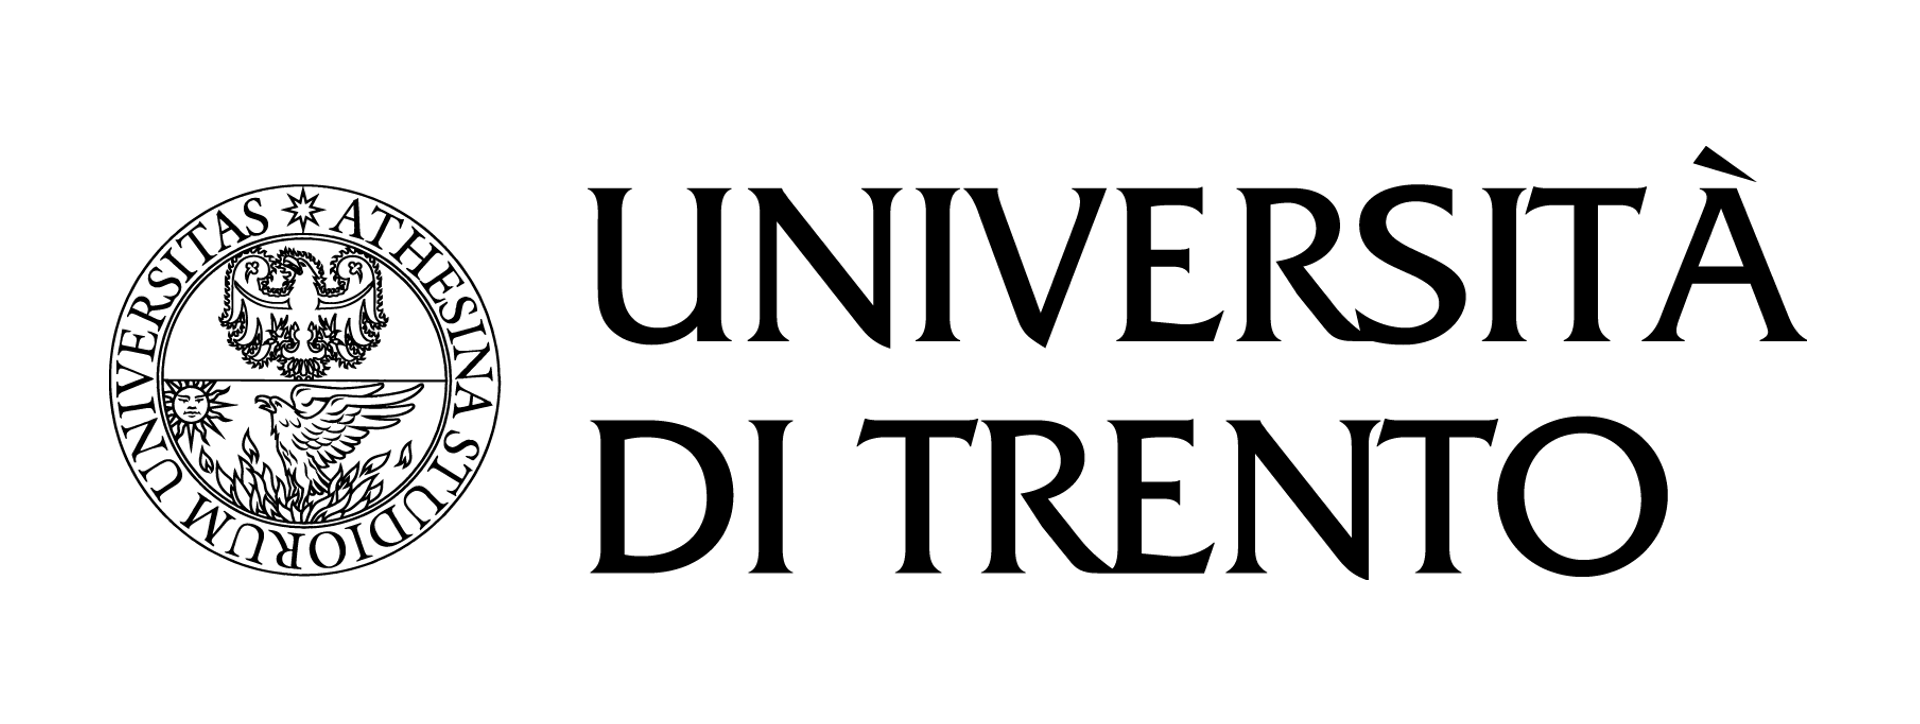
\includegraphics[scale=0.15]{immagini/logo-unitn.png}
    \maketitle
\end{figure}
\begin{center}\textbf{
    Corso di Laurea in Ingegneria Industriale\\
    Corso di {Sistemi Meccanici e Modelli}\\
    Anno accademico: 2021/2022}
\vspace{2cm}
\begin{abstract}\centering
Lo scopo di questo progetto è lo studio cinematico e il dimensionamento idraulico di una trinciaerba interfilare utilizzata nella coltivazione intensiva di viti e alberi da frutto in genere.
\end{abstract}
\end{center}
\thispagestyle{empty}
\newpage
%%%%%%%%%%%%%%%%%%%%%%%%%%%%%%%%%%%%%%%%%%%%%%%%%%%%%%%%%%%%%%%%%%%%%%%%%%%%%%%%%%%%
\tableofcontents
\listoffigures
\thispagestyle{empty}
\newpage
%%%%%%%%%%%%%%%%%%%%%%%%%%%%%%%%%%%%%%%%%%%%%%%%%%%%%%%%%%%%%%%%%%%%%%%%%%%%%%%%%%%%
\setcounter{page}{3}
\section{Scopo del progetto e requisiti }
\subsection{Funzioni e obiettivi dei trinciaerba interfilari}
  Il trinciaerba è un attrezzo utilizzato in campo agricolo nelle operazioni di diserbo delle coltivazioni intensive di alberi da frutto. Esso permette sia di rimuovere la vegetazione tra due piante nella zona al disotto del filare (detta "interfila") sia di estirpare i "polloni", germogli che si formano alla base della pianta e risultano dannosi per l'attività fruttifera della stessa. Le applicazioni classiche sono uliveti e vigneti, il progetto è rivolto a studiare quest'ultimi.\\
  Questa attrezzatura consente di velocizzare i tempi di sfalcio di erba e germogli automatizzando tali attività, permettendo così un risparmio di tempi e manodopera. Ricordiamo infine l'eco-compatibilità della lavorazione perché sostituisce l'utilizzo di diserbanti chimici e altri prodotti fitosanitari, dannosi per l'ambiente.\\
  A seconda del modello, può essere agganciato alla parte anteriore o posteriore di un mezzo mobile -ad esempio un trattore- ed è ad esso collegato per ricevere la potenza meccanica necessaria al funzionamento. Durante l'avanzamento tra i filari, si ha lo sfalcio dell'erba e la potatura dei germogli attraverso un tamburo rotante nel quale sono inseriti degli spaghi di materiale plastico abbastanza flessibili ma al contempo resistenti.\\
  Il tamburo rotante è montato su un braccio mobile ed esegue un movimento ciclico di avvicinamento e allontanamento delle piante.\\
  Durante lo sfalcio, il rullo deve lavorare l'interfila tra le piante ma al contempo deve essere in grado di aggirarle rapidamente quando vi giunge in prossimità per non urtarle. Ciò è permesso da un tastatore, ovvero una "bacchetta" di metallo solidale al tamburo che lo precede. Al contatto con un ostacolo, l'elemento sensibile ruota attorno a un fulcro e tale torsione aziona un leveraggio che mette in comunicazione sistema meccanico e idraulico. A questo punto l'azionamento di una valvola distributrice permette la retrazione di un pistone collegato al braccio mobile e il conseguente movimento permette di aggirare la pianta.\\
  Nelle immagini alla pagina seguente, si possono vedere sia dei modelli di trinciaerba attualmente in produzione (nella figura \ref{triniaerba_internet}) sia di un modello degli anni '80 (figura \ref{aratro}).\\
  Durante il progetto ci siamo rifatti ad entrambe le generazioni di macchina.
  
\begin{figure}[H] 
\centering 
\includegraphics[scale=1]{immagini/trinciaerba_1.jpg}

\label{triniaerba_internet}
\end{figure}

\subsection{Parametri di conformazione dell'ambiente di utilizzo}
Come già detto questa attrezzatura può essere impiegata in tutte le tipologie di coltivazione intensiva di frutteti ma in questa relazione si fa particolarmente riferimento alle viti, poiché tipiche delle zone da cui noi componenti del gruppo proveniamo. \\
La distanza tra due piante, misurata su un vigneto di pianura, è di 1.60 (\si{\meter}). La distanza tra due filari è di 2.80 (\si{\meter}). La lunghezza del filare non è un parametro influente nello studio del movimento compiuto dagli organi idraulici.\\
Le lavorazioni eseguite dal macchinario vengono effettuate nelle stagioni primaverili ed estive quindi,  nella scelta dell'olio, bisognerà tenere conto del fatto che le temperature ambientali possono attestarsi su valori abbastanza elevati.

\newpage
%%%%%%%%%%%%%%%%%%%%%%%%%%%%%%%%%%%%%%%%%%%%%%%%%%%%%%%%%%%%%%%%%%%%%%%%%%%%%%%%%
\section{Analisi meccanica}
\subsection{Dimensione tamburo rotante}
Facendo riferimento a cataloghi si possono ottenere le dimensioni del tamburo: un cilindro forato di acciaio dal diametro esterno di 100\ (\si{\milli\meter}), diametro interno di 90\ (\si{\milli\meter}) e lunghezza 520 \ (\si{\milli\meter}):
\begin{gather}
    m=\frac{\pi \cdot (D^2-d^2) \cdot L \cdot \rho}{4}=\frac{\pi \cdot (0.1^2-0.09^2) \cdot 0.520 \cdot 7800}{4} = 6.05 \ \ (\si{\kilo\gram})
    \label{Massa_tamburo}\\
    J=\frac{m\cdot (R^2+r^2)}{2}=\frac{6.05\cdot (0.050^2+0.045^2)}{2} = 1.37 \cdot 10^{-2} \ \ (\si{\kilo\gram \square \meter})
    \label{inerzia_tamburo}
\end{gather}\\
Sul tamburo vengono montati degli spaghi di materiale plastico che materialmente effettuano lo sfalcio. Quest' ultimi hanno una lunghezza pari a 100 (\si{\milli\meter}).\\ 
Possiamo quindi considerare l'ingombro totale della parte che effettua la lavorazione come il volume occupato da un cilindro di lunghezza 520 (\si{\milli\meter}) e diametro 300 (\si{\milli\meter}). Durante lo sfalcio la distanza tra estremità del tamburo e terreno è di 100 (\si{\milli\meter}). \\


Il movimento che deve compiere il braccio porta attrezzo è un ciclo suddiviso in due fasi:
\begin{itemize}
	\item fase di lavoro: il pistone è nelle posizione di apertura massima ed il braccio effettua la lavorazione della parte di filare lontana dalle piante formando un angolo di 45\si{\degree} con esse;
	\item fase di spostamento: il braccio viene retratto per evitare l'urto con la pianta e riposizionato in centro al filare una volta superata. L'angolo formato tra la normale al filare e braccio al momento di massimo spostamento di quest'ultimo è di 69\si{\degree}.
	\end{itemize} 

Dai dati su distanza tra piante e velocità di movimento della macchina possiamo calcolare il tempo in cui deve essere completato il ciclo di lavoro:
\begin{equation}
t \ped{TOT} = \frac{s}{v} \ \  (s)
\label{t_TOT_1}
\end{equation}
Con:

Riportiamo nelle seguenti tabelle i valori numerici dei parametri e delle equazioni appena enunciate in forma letterale:
\begin{table}[H]
\centering
\begin{tabular}{ |c|c|c|c|c|c|c|c|c| } 
\hline
 Parametro & Simbolo & Valore & U.D.M   \\ 
 & &  &\\
 Velocità movimento trattore & v & 2.5 & (\si{\kilo \meter \per \hour})   \\ 
Spazio tra due piante & s & 1.6 & (\si{\meter})  \\
 Diametro tamburo+spaghi & b & 0.3 &  (\si{\meter})  \\
 Anticipo bacchetta & d & 0.1 & (\si{\meter})  \\
Lunghezza tamburo & a & 0.520 & (\si{\meter})  \\
 Frazione rientro & - & 0.6 & -  \\
 Frazione uscita & - & 0.4 & -  \\
 Corsa pistone & c & 0.046 & (\si{\meter})  \\
 \hline
\end{tabular}
\caption{Parametri geometrici movimento braccio}
    \label{tab_geometrici_braccio}
\end{table}
\medskip


\includepdf[pages=4, scale=.65,pagecommand={\subsection{Tabella caratteristiche filtrazione olio}\label{Tabella_olio}},linktodoc=true] {schede_tecniche/scheda_ISO_4406.pdf}

\end{document}
